This is an open source project under license \cite{gplv3}. \\

\chapter{Introduction}

Sign or signed languages are complete natural languages that are expressed visually.
They have their own grammar and lexicon and they are not universal. \\ 

Sign languages have became the main way of communicating between deaf and dumb people. Nevertheless,
it is not common in society to be able to understand them, so the gap between these communities
and the rest of society have increased since years. \\

As a future Software Engineer, I have a big social responsability, because my developments and ideas
may help minorities and lessen gaps like this one. \\

Solutions such as a videocall application, that subtitles sign languages, could make sign language 
speakers be able to communicate with non-signers.
Although there are a lot of dictionaries and applications to learn sign language, there is an 
absence of applications that verify how you perform signing.
Learning sign language would be easier and more accessible if you would not need someone to do this verification,
and devices are now able to do this.

\section{Preliminar analysis. Viability study.}

In order to create an application to verify a signs or a videocall app, 
translating signs into text would be neccessary. \\

Past works have their main focus in translating signs into text using special gloves. Although this is effective 
and would solve the problem, not everyone could afford these gloves, and the entrance to sign would be so expensive 
that people would not feel attracted to this field. \\

The most accessible hardware for users would be the integrated cameras in their phones and pc's. Therefore,
the main objective of this initial study would be to analyse the efficiency and viability of translating 
a video into text without any complex hardware.

\subsection{Sign language characteristics}
The first thing that comes into mind is to develop a deep learning model able to translate signed sentences into 
text. Firstly, we should know the difficulties that this would take:
\begin{itemize}
    \item In order to be able to translate a signed sentence into text, the model should understand the context to formulate the sentence correctly.
    \item Some words are signed the same way.
    \item Signs are performed differently if you are left-handed or right-handed.
    \item The dataset should contain videos of people from different ethnics, sex, race, etc signing, as it should be used by everyone.
\end{itemize}

Just analysing the alphabet would be much easier, as all letters are signed statically (in ASL: American Sign Language), except two.
Therefore, a classification deep learning model could be developed and validate the images/videos from the user.
Nevertheless, this has not that relevance, as it has already been developed and implemented by some applications such as Snapchat.

\subsection{Literature review}
\begin{longtable}{|p{3cm}|p{4cm}|p{6cm}|}
    \hline {Type} & {Title} & {Note}      \\
    \hline Video & La INFRAESTRUCTURA detrás de TikTok \cite{TikTok2021} & Infraestructure analysis. How to divide a big service into smaller ones and create an UML diagram from it \\
    \hline Journal & Word-level Deep Sign Language Recognition from Video: A New Large-scale Dataset and Methods Comparison \cite{Li2019} & They introduce a large scale dataset for American Sign Language, consisting of 2000 words performed by more than 100 signers in more than 20.000 videos. They also introduce two models and compare them: holistic visual appearance-based approach, and 2D human pose based approach. \\
    \hline Journal & Recognition of user-dependent and independent static hand gestures: Application to sign language \cite{Sadeddine2021} & Sign recognition becomes a very complex tax due to heterogeneous environment. This article study how to improve accuracy of models using static hand gesture recognition based on a set of image descriptors: Gradient Local Auto-Correlation (GLAC), Gabor Wavelet Transform (GWT), and Fast Discrete Curve Transform (FDCT). \\
    \hline Journal & Optimization of convolutional neural networks architectures using pso for sign language recognition \cite{Fregoso2021} & It presents an approach to design convolutional neural network architectures, using the particle swarm optimization algorithm.\\
    \hline Webpage & TSPNet: Hierarchical Feature Learning via Temporal Semantic Pyramid for Sign Language Translation \cite{SLTTSPNet} & The repository contains the implementation of TSPNet \\
    \hline Journal & Visual Alignment Constraint for Continuous Sign Language Recognition \cite{Min2021} & How to solve the overfitting problem in recent CTC-based CSLR worksdue to the insufficient training of the feature extractor using a Visual Alignment Constraint (VAC) to enhance the feature extractor with more alignment supervision \\
    \hline Webpage & Visual Alignment Constraint for Continuous Sign Language Recognition \cite{Min2021} & GitHub repository for the paper above \\
    \hline Journal & ELM based two-handed dynamic Turkish Sign Language (TSL) word recognition \cite{ELM2021} & It studies the recognition of dynamic words in Turkish Sign Language (TSL) with two hands was studied using the Leap Motion Controller (LMC) device \\
    \hline Journal & Applying deep neural networks for the automatic recognition of sign language words: A communication aid to deaf agriculturists \cite{Venugopalan2021} & In order to help deaf agriculturists, they propose a model using LSTM and trained using a small dataset of the most common indian signed-words in this field \\
    \hline Journal & Real-Time Sign Language Detection using Human Pose Estimation \cite{Moryossef2020} & Lightweight real-time sign language detection model for future use in videocall applications \\
    \hline Report  & Sign Language Transformers: Joint End-to-end Sign Language Recognition and Translation \cite{SignLanguageTransformers} & New architecture for continuous sign language recognition \\
    \hline Journal & Sign Language Recognition Using ConvolutionalNeural Networks \cite{Bronstein2015} & Their contribution considers a recognition system using the Microsoft Kinect,convolutional neural networks (CNNs) and GPU acceleration \\
    \hline Video   & Real-Time Sign Language Detection for Video Conferencing Applications \cite{RT2021} & In order to create a videoconferencing app and situate as main signer the person who is signing, the author proposes to use a noise that people are not able to hear. That way, the apps are mislead and videoconferencing between deaf people is possible \\
    \hline Webpage & American Sign Language Recognition in Python using Deep Learning \cite{ASLRecognitionPython} & Model that uses knowledge transfer to recognise letters in ASL \\
    \hline Webpage & How to use transfer learning for sign language recognition \cite{Vagdevi2019} & From ResNet, model using knowledge transfer that achieves  percent accuracy in a test environment \\ 
    \hline Webpage & How to build a convolutional neural network that recognizes sign language gestures \cite{Vagdevi2019i} & Neural network to recognise letters in ASL \\
    \hline Journal & Sign Language Recognition for Computer Vision Enthusiasts \cite{Vaishshells2021} & Two models to recognise letters. One static and one dynamic using an american sign language dataset \\
    \hline Journal & ASL Alphabet \cite{Akash2018} & Dataset to sign letters in ASL. It transforms the letters 'J' and 'Z' into images, due that they are signed dynamically and video recognition would be neccessary. This way, just image classification could be used \\
    \hline Webpage & Hands-On Guide To Sign Language Classification Using CNN \cite{SignLanguageClassification2020} & Model to classify letters in ASL. It just classify static letters (all except 'J' and 'Z') \\
    \hline Journal & Sign Language Recognition: A Deep Survey \cite{Rastgoo2021} & State of art summary. It contains links to main model, datasets and architectures \\
    \hline Video   & Sign Language Detection using ACTION RECOGNITION with Python | LSTM Deep Learning Model \cite{SignLanguageRecognitionUsingActionRecognition} & Classify some ASL signs from a webcam \\
    \hline Video   & Real Time Sign Language Detection with Tensorflow Object Detection and Python | Deep Learning SSD \cite{SignLanguageRecognitionUsingObjectDetection} & App to recognise 5 static signs. It teaches how to create a dataset, label images and train a model from a dataset \\
    \hline Video   & Building a Real Time Sign Language Detection App with React.JS and Tensorflow.JS | Deep Learning \cite{SignLanguageRecognitionUsingReactjsAndTensorflow} & Transform a python model to a tensorflow model. Upload it to the cloud and download it on the frontend, so that we can use it using a React.js app to validate videos on the frontend \\
    \hline Journal & Deep Learning Techniques for Spanish Sign Language Interpretation \cite{SpanishDataset2021} & Dataset for Spanish Sign Language recognition. It proposes to use CNN to classify static letters and RNN to classify dynamic letters. \\
    \hline
    \caption{Literature review}
    \label{table:introduction_literature_review}
\end{longtable}

\subsection{Solution to implement's selection}
As I found in the literature a good dataset of American Sign Language \cite{Li2019}, my investigation will use this dataset. \\

A videocall application, or integrating a model into an existing application such as Jitsi, would be a very hard task due to my lack of knowledge in the deep learning field and that I don't really know if the model will perform correctly. \\ 

As I found an existing and pretrained model that translates videos of people signing into text, I would opt to do an application to learn American Sign Language. I would integrate this model in the application so that the user can sign and the app automatically verifies if the sign is performed correctly.

\subsubsection{In depth: WLASL: A large-scale dataset for Word-Level American Sign Language}
Due to the importance of American Sign Language for the deaf community, and the lack of a huge dataset \\
that allows recognition at a word-level and a sentence-level, WLASL was created. 

\paragraph{Characteristics}
They provide a big dataset, which characteristics are:
\begin{itemize}
    \item It is composed only by \textbf{monocular-RGB} videos: the videos do not rely on special equipment, such as depth cameras, colored gloves...
    \item All signers are in near-frontal views.
    \item The dataset contains 21.083 videos.
    \item Each video contains one sign in ASL.
    \item The videos are performed by 119 signers.
    \item Each sign is performed by at least 3 different signers.
    \item The duration of the videos range from 0.36 to 8.12 seconds. The average is 2.41 seconds. The average intra-class standard deviation of the videos is 0.85 seconds.
\end{itemize}

\paragraph{Importance of this dataset}
Due to the lack of a standard dataset, I cannot compare existing models. They are trained using small-datasets \\
and I can not trust their effectiveness in a real environment. Therefore, that's why this project is so \\
important, because the dataset is big enough and has a conditions that allow to train a model that can \\
be used in a real environment without special equipment by the user.

\paragraph{Subdivisions of the dataset}
The dataset is divided in 4 parts, so that I can train a model in every dataset and select the model depending on the word that I try to classify.
\begin{table}[h]
    \centering
    \resizebox{\textwidth}{!}{
    \begin{tabular}{|c|c|c|c|c|c|}
        \cline{1-6}  Datasets   & Gloss &  Videos &  Mean  & Signers   & Year       \\
        \hline       WLASL100   &   100 &   2,038 &  20.4  &      97   & 2019       \\
        \hline       WLASL300   &   300 &   5,117 &  17.1  &     109   & 2019       \\
        \hline      WLASL1000   &  1000 &  13,168 &  13.2  &     116   & 2019       \\
        \hline      WLASL2000   &  2000 &  21,083 &  10.5  &     119   & 2019       \\
        \hline
    \end{tabular}
    }
\caption{Subdivisions of the dataset}
\label{table:introduction_dataset_subdivisions}
\end{table}

\paragraph{Models proposed} The paper proposes two models trained on this dataset:
\begin{itemize}
    \item I3D: it follows a I3D network architecture. It is trained using ImageNet \cite{ImageNet} \\ 
    and finetuned using Kinetics-400 \cite{Kinetics400}. Since the class number varies depending on \\
    the dataset, the last classification layer is changed according to it. \\
    \begin{figure}[H]
        \begin{center}
            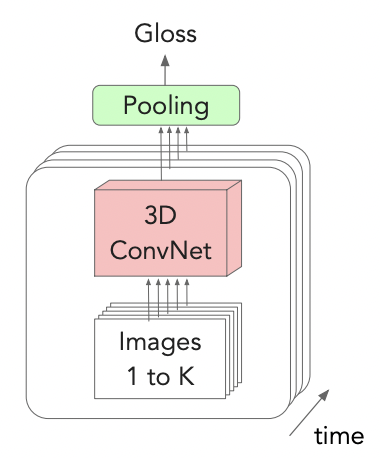
\includegraphics[width=0.4\textwidth]{assets/i3d.png}
            \caption{I3D architecture}
            \label{fig:introduction_i3d}
        \end{center}
    \end{figure}
    \item Pose TGCN: pose based temporal graph neural network. Usually, motion is modelled using 2D joint angles. \\
    They encode the motion using a holistic representation of the trajectories of body keypoints. They represent \\
    the human body as a fully-connected graph to learn the dependencies between joints in the trajectories. \\
    \begin{figure}[H]
        \begin{center}
            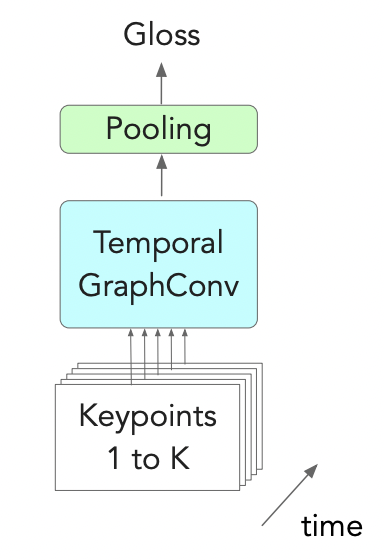
\includegraphics[width=0.4\textwidth]{assets/tgcn.png}
            \caption{TGCN architecture}
            \label{fig:introduction_tgcn}
        \end{center}
    \end{figure}
\end{itemize}

\subparagraph{Data pre-processing} They following transformations are applied:
\begin{itemize}
    \item Resize the original resolution so the bounding-box of the signer is 256 pixels.
    \item Crop a 224x224 patch from an input frame.
    \item Apply an horizontal flipping with a prob of 0.5
\end{itemize}

\subparagraph{Implementation details and accuracy evaluation} The models are all implemented in Pytorch. \\
Models accuracy (top-10): \\
\begin{figure}[!ht]
    \begin{center}
        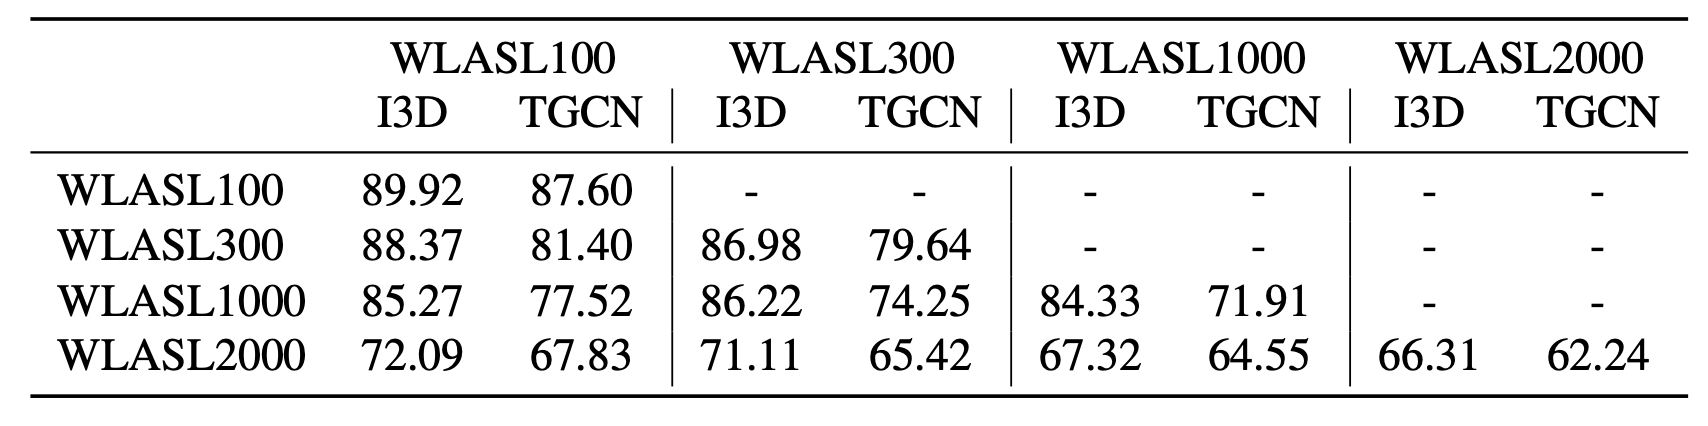
\includegraphics[width=1.0\textwidth]{assets/models_accuracy.png}
        \caption{Models' accuracy comparison}
        \label{fig:introduction_model_accuracy_comparison}
    \end{center}
\end{figure}
\\

Due to the better performance of the I3D model, I use it in my implementation.
